\chapter{Biologia do câncer}\label{ch:b3:cancer-biology}

Um \omterm{def:b3:cancer-biology:hallmarks}{tumor} grande o bastante para ser apalpado, de um centímetro, contém
um bilhão de células e é obra de cerca de trinta duplicações a partir
de uma célula que deu errado --- tipicamente uma década de crescimento
antes que alguém soubesse. Atrás dessa célula estão várias mutações,
cada uma das quais teve de ocorrer na mesma linhagem e cada uma das
quais removeu um dos controles dos dois capítulos anteriores: um freio
da divisão, um gatilho de morte, um limite do número de divisões, a
obrigação de ficar no lugar. O \omterm{def:b3:cancer-biology:hallmarks}{câncer} é a evolução de uma população de
células dentro de um corpo, por mutação e seleção, rumo a um estado que
serve às células e mata o organismo. Este capítulo trata dos genes que
são atingidos e do que eles normalmente fazem, da estatística que
revela quantos golpes são necessários, da fisiologia que um \omterm{def:b3:cancer-biology:hallmarks}{tumor}
precisa adquirir para crescer além de um milímetro e para se espalhar,
das causas que se pode evitar, e das terapias --- de venenos que matam
células em divisão a anticorpos que soltam o sistema imune --- que a
biologia tornou possíveis, junto com a razão evolutiva pela qual elas
tantas vezes falham.

\section{O que é um câncer}

\begin{definition}[Tumor, câncer, marcas]\label{def:b3:cancer-biology:hallmarks}
\index{câncer}\index{tumor}\index{maligno}\index{metástase}\index{marcas do câncer}
Um \emph{tumor} (neoplasia) é um clone de células que escapou dos
controles de seu crescimento e se acumula num tecido. Ele é
\emph{benigno} se permanece confinado e encapsulado, e \emph{maligno}
--- um \emph{câncer} --- se suas células invadem o tecido vizinho e
semeiam tumores secundários em outros lugares (a \emph{metástase}), que
é o que mata. Os cânceres são nomeados pela célula de origem: os
carcinomas vêm dos epitélios (\qty{85}{\%} dos cânceres humanos), os
sarcomas do tecido conjuntivo, as leucemias e os linfomas das células
formadoras do sangue, os gliomas da glia. Seja qual for o tecido, um
clone maligno adquiriu o mesmo conjunto de capacidades, as \emph{marcas
do câncer}: ele prolifera sem sinais externos de crescimento e ignora
os sinais que o deteriam; resiste à \omterm{def:b3:cell-cycle-apoptosis:apoptosis}{apoptose}; divide-se sem limite,
tendo reativado a \omterm{def:b3:cancer-biology:telomerase}{telomerase}; induz vasos sanguíneos; invade e
metastatiza; e, por baixo de tudo isso, seu genoma é instável, ele
reprograma seu metabolismo rumo à glicólise mesmo na presença de
oxigênio (o efeito Warburg), recruta células inflamatórias que o
ajudam, e escapa do sistema imune. Cada marca é um controle do tecido
normal derrotado, e cada uma corresponde a genes.
\end{definition}

\begin{omfigure}
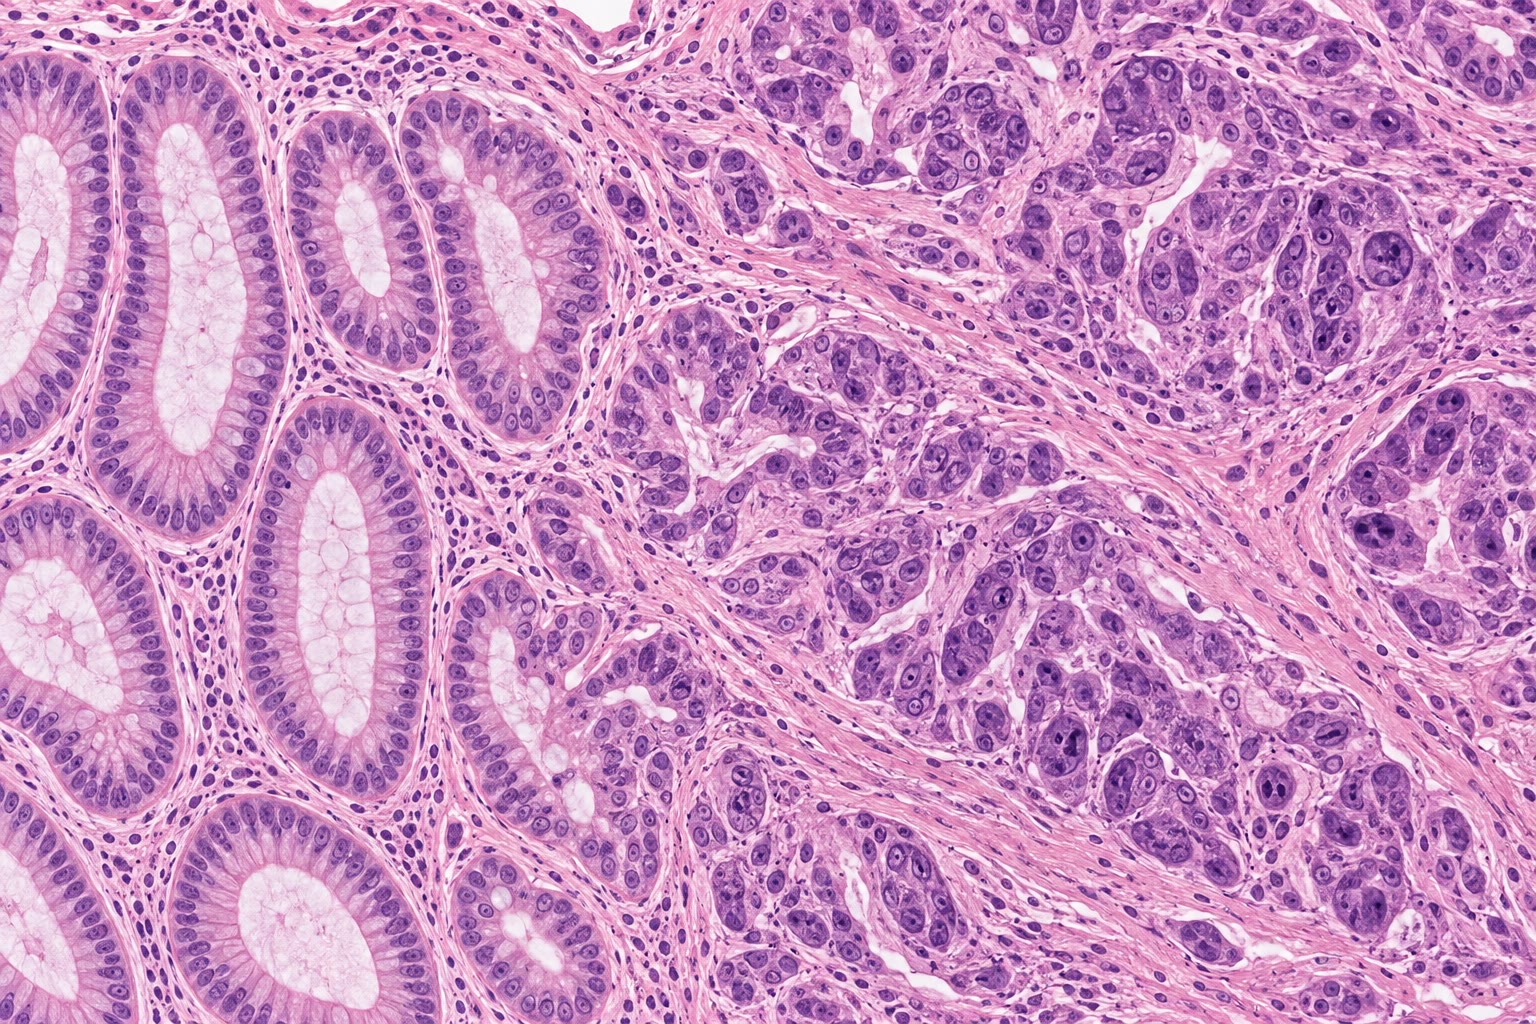
\includegraphics[width=0.56\linewidth]{images/book5/ai/b5-11-tumour-histology.jpg}

{\small Um carcinoma em sua borda: à esquerda, epitélio glandular
ordenado, com núcleos regulares; à direita, células amontoadas, de
núcleos grandes e irregulares, invadindo o estroma subjacente --- a
imagem que um patologista lê para chamar um \omterm{def:b3:cancer-biology:hallmarks}{tumor} de \omterm{def:b3:cancer-biology:hallmarks}{maligno}.}
\end{omfigure}

\section{Os genes que são atingidos}

\begin{definition}[Oncogenes e supressores de tumor]\label{def:b3:cancer-biology:genes}
\index{oncogene}\index{proto-oncogene}\index{gene supressor de tumor}\index{Ras}\index{p53}\index{hipótese dos dois golpes}
Um \emph{proto-oncogene} é um gene normal que promove a proliferação ou
a sobrevivência --- um fator de crescimento, seu receptor, uma proteína
de sinalização, um fator de transcrição, uma \omterm{def:b3:cell-cycle-apoptosis:cdk}{ciclina} --- e um
\emph{oncogene} é uma forma mutante que fica ativa sem seu sinal
normal: uma mutação pontual que trava a \omterm{def:b3:membrane-traffic:coats}{GTPase pequena} \emph{Ras} em
seu estado ligado a GTP (a glicina~12 num quarto de todos os \omterm{def:b3:cancer-biology:hallmarks}{cânceres}),
uma amplificação do gene do receptor HER2 ou do fator de transcrição
Myc, uma translocação que funde o \emph{BCR} à cinase \emph{ABL} na
leucemia mieloide crônica ou põe o \emph{MYC} ao lado de um
intensificador de anticorpo no linfoma de Burkitt. Um alelo mutante
basta: os oncogenes agem de modo dominante. Um \emph{gene supressor de
\omterm{def:b3:cancer-biology:hallmarks}{tumor}} contém a proliferação ou impõe a morte ou o reparo --- a Rb e a
p16 no \omterm{def:b3:cell-cycle-apoptosis:checkpoints}{ponto de restrição}, a \emph{p53}, a guardiã que detém ou mata
uma célula danificada, a APC na \omterm{prop:b3:cancer-biology:pathways}{via Wnt} do cólon, a PTEN, a BRCA1 e a
BRCA2, os genes de \omterm{prop:b3:dna-repair:fidelity}{reparo de mau pareamento} --- e precisa perder os
dois alelos para contribuir: \emph{dois golpes}, o primeiro muitas
vezes herdado nas síndromes de \omterm{def:b3:cancer-biology:hallmarks}{câncer} familiar, o segundo somático. A
\emph{p53} está mutada em metade de todos os \omterm{def:b3:cancer-biology:hallmarks}{cânceres} humanos e sua via
está desativada na maior parte do resto.
\end{definition}

\begin{proof}[Evidência]
Rous (1911) transmitiu um sarcoma de galinha com um filtrado livre de
células, um vírus, cujo único gene transformante, o \emph{src}, foi
mostrado por Varmus e Bishop (1976) ser uma cópia capturada de um gene
normal da galinha --- os \omterm{def:b3:cancer-biology:genes}{oncogenes} são genes celulares alterados.
Weinberg (1982) transferiu DNA de um carcinoma humano de bexiga para
células de camundongo em cultura, que se transformaram; o fragmento
responsável era o \emph{RAS} com uma única troca de base, e a mesma
troca estava ausente do tecido normal do paciente. Knudson (1971)
comparou crianças com o \omterm{def:b3:cancer-biology:hallmarks}{tumor} ocular retinoblastoma: as que tinham
história familiar desenvolviam vários \omterm{def:b3:cancer-biology:hallmarks}{tumores} nos dois olhos, cedo; as
que não tinham desenvolviam um, mais tarde --- coerente com a
necessidade de um evento somático nos casos familiares e de dois nos
esporádicos, e assim com um gene cujas duas cópias precisam ambas ser
perdidas. O \emph{RB} foi clonado em 1986, e os dois alelos estavam de
fato inativados em cada \omterm{def:b3:cancer-biology:hallmarks}{tumor}.
\end{proof}

\begin{theorem}[Golpes e a curva de idade]\label{thm:b3:cancer-biology:armitage-doll}
\index{modelo de Armitage--Doll}\index{carcinogênese em múltiplas etapas}
Suponha que um \omterm{def:b3:cancer-biology:hallmarks}{câncer} exija $k$ eventos independentes e limitantes da
taxa numa mesma linhagem celular, cada um ocorrendo a uma taxa
constante $u$ por célula por ano, numa população de $N$ células
suscetíveis, com $ut \ll 1$. Então a probabilidade de uma dada célula
ter sofrido todos os $k$ eventos até a idade $t$ é de cerca de
$(ut)^{k}$, o risco cumulativo no tecido é de cerca de $N(ut)^{k}$, e a
incidência --- casos novos por ano na idade $t$ --- é
\[
I(t) \approx N\,k\,u^{k}\,t^{\,k-1},
\]
uma potência da idade com expoente $k - 1$: uma reta de inclinação
$k - 1$ num gráfico log--log. Para uma pessoa que herda um dos eventos,
o mesmo \omterm{def:b3:cancer-biology:hallmarks}{câncer} tem incidência $\propto t^{\,k-2}$, uma potência abaixo.
\end{theorem}
\begin{proof}
Cada evento, à taxa $u$, ocorreu até o instante $t$ com probabilidade
$1 - e^{-ut} \approx ut$; os eventos são independentes, de modo que
todos os $k$ ocorreram com probabilidade $(ut)^{k}$, e a ordem em que
ocorreram não importa aqui. Com $N$ células e eventos raros, o número
esperado de células que completaram a sequência é $N(ut)^{k}$, e a
incidência é sua derivada temporal, $Nku^{k}t^{k-1}$. Herdar um evento
deixa $k - 1$ por ocorrer: $(ut)^{k-1}$, incidência $\propto t^{k-2}$.
Se a ordem dos eventos importasse (só $1$ entre $k!$ ordens levasse ao
\omterm{def:b3:cancer-biology:hallmarks}{câncer}), o prefator mudaria, não o expoente.
\end{proof}

\begin{example}[Ler o expoente]\label{ex:b3:cancer-biology:exponent}
A incidência da maioria dos carcinomas em adultos sobe como cerca da
quinta à sexta potência da idade --- de cerca de $1$ em \num{100000}
por ano aos trinta a $1$ em $300$ aos oitenta, um fator de $300$ para
um fator $2.7$ na idade, e $2.7^{5.7} \approx 300$ ---, o que sugere
seis ou sete eventos limitantes da taxa. A estimativa é grosseira: a
expansão de um clone depois de cada golpe eleva o número de células sob
risco do golpe seguinte, de modo que menos eventos com crescimento
clonal entre eles dão a mesma inclinação, e o número de mutações
\emph{condutoras} encontradas em \omterm{def:b3:cancer-biology:hallmarks}{tumores} sequenciados é de duas a oito.
O retinoblastoma de Knudson se encaixa exatamente na segunda afirmação
do teorema: a doença esporádica, que precisa de dois golpes, tem uma
incidência que sobe com a idade (ao longo dos poucos anos em que os
retinoblastos existem); a doença hereditária, que precisa de um, está
presente a uma taxa quase constante desde o nascimento e ataca cedo e
repetidamente.
\end{example}

\begin{omfigure}
\begin{tikzpicture}
\begin{axis}[
  width=0.68\linewidth, height=6cm,
  xmode=log, ymode=log,
  xmin=20, xmax=100, ymin=1e-6, ymax=1e-1,
  xlabel={idade (anos)}, ylabel={incidência por pessoa por ano},
  xlabel style={font=\small, at={(axis description cs:0.5,-0.12)}, anchor=north},
  ylabel style={font=\small},
  tick label style={font=\small}, xtick={20,30,50,80}, xticklabels={20,30,50,80},
  clip=false,
]
\addplot[very thick, omThm, domain=20:100, samples=2] {1e-5*(x/30)^5.7};
\addplot[very thick, omDef, domain=20:100, samples=2] {3e-4*(x/30)^1};
\addplot[very thick, omMeth!70!black, domain=20:100, samples=2] {2e-3};
\node[font=\scriptsize, omThm, anchor=south west] at (axis cs:38,2.5e-6) {carcinomas: inclinação $5$--$6$, seis ou sete eventos};
\node[font=\scriptsize, omDef, anchor=south west] at (axis cs:22,6e-4) {dois golpes: inclinação 1};
\node[font=\scriptsize, omMeth!70!black, anchor=south west] at (axis cs:22,2.3e-3) {um golpe herdado: inclinação 0};
\end{axis}
\end{tikzpicture}

{\small Incidência contra idade em eixos logarítmicos. Um \omterm{def:b3:cancer-biology:hallmarks}{câncer} que
precisa de $k$ eventos limitantes da taxa sobe como $t^{k-1}$: a reta
íngreme dos carcinomas do adulto e os dois casos de Knudson --- um
\omterm{def:b3:cancer-biology:hallmarks}{tumor} de dois golpes subindo linearmente e o mesmo \omterm{def:b3:cancer-biology:hallmarks}{tumor} num portador
de um golpe herdado, a uma taxa constante desde o nascimento.}
\end{omfigure}

\begin{proposition}[As vias que são atingidas]\label{prop:b3:cancer-biology:pathways}
\index{via Ras--MAPK}\index{via PI3K}\index{via Wnt}
As centenas de genes de \omterm{def:b3:cancer-biology:hallmarks}{câncer} se distribuem por uma dúzia de vias,
cada uma das quais um \omterm{def:b3:cancer-biology:hallmarks}{tumor} desativa em algum ponto. As vias dos
fatores de crescimento: um receptor com atividade tirosina-cinase
(EGFR, HER2), a \omterm{def:b3:cancer-biology:genes}{Ras}, a cascata de cinases Raf--MEK--ERK até o núcleo e,
em paralelo, PI3K--Akt--mTOR rumo à sobrevivência e ao crescimento,
contida pela PTEN; um \omterm{def:b3:cancer-biology:hallmarks}{tumor} ativa uma delas, por meio de qualquer dos
genes. O freio do \omterm{def:b3:cell-cycle-apoptosis:cdk}{ciclo celular}: \omterm{def:b3:cell-cycle-apoptosis:cdk}{ciclina} D, Cdk4, p16, Rb
(\cref{ch:b3:cell-cycle-apoptosis}). A guardiã: a \omterm{def:b3:cancer-biology:genes}{p53} e seus
reguladores. A morte: a Bcl-2. A sinalização do desenvolvimento: Wnt
(APC, $\beta$-catenina) no cólon, Hedgehog na pele e no cérebro, Notch
nos linfócitos~T. A manutenção do genoma: o \omterm{prop:b3:dna-repair:fidelity}{reparo de mau pareamento}, a
\omterm{def:b3:dna-repair:dsb}{BRCA}, a \omterm{def:b3:dna-repair:ddr}{ATM}. A \omterm{def:b3:chromatin-epigenetics:nucleosome}{cromatina}: os \omterm{def:b3:chromatin-epigenetics:histone-code}{escritores} e remodeladores do
\cref{ch:b3:chromatin-epigenetics}, mutados num terço dos \omterm{def:b3:cancer-biology:hallmarks}{tumores}. A
imortalidade: o promotor da \omterm{def:b3:cancer-biology:telomerase}{telomerase}. Como uma via é uma série de
etapas, as mutações em genes diferentes são alternativas --- um \omterm{def:b3:cancer-biology:hallmarks}{tumor}
com \omterm{def:b3:cancer-biology:genes}{Ras} mutante raramente tem também EGFR mutante --- e fármacos contra
uma etapa podem ser derrotados por uma mutação a jusante.
\end{proposition}

\begin{omfigure}
\begin{tikzpicture}[every node/.style={font=\scriptsize}, >=stealth]
  % membrane
  \draw[very thick, omDef] (0,3.6) -- (12,3.6); \draw[very thick, omDef] (0,3.3) -- (12,3.3);
  \node[above] at (1.0,3.65) {exterior}; \node[below] at (1.0,3.25) {citosol};
  % receptor
  \draw[thick, fill=omProp!35] (3.7,3.0) rectangle (4.1,4.1); \draw[thick, fill=omProp!35] (4.3,3.0) rectangle (4.7,4.1);
  \node[above, align=center] at (4.2,4.15) {fator de crescimento $\to$ receptor cinase\\(EGFR, HER2)}; \node[right, omThm, font=\tiny] at (4.75,4.0) {amplificado};
  % Ras
  \node[draw, thick, rounded corners, fill=omDef!20] (ras) at (4.2,2.3) {Ras--GTP};
  \node[right, omThm, font=\tiny] at (5.0,2.3) {G12: sempre ligada};
  \node[draw, thick, rounded corners, fill=omDef!20] (raf) at (4.2,1.4) {Raf $\to$ MEK $\to$ ERK};
  \node[right, omThm, font=\tiny] at (5.8,1.4) {BRAF V600E};
  \node[draw, thick, rounded corners, fill=omMeth!25] (myc) at (4.2,0.4) {Myc, ciclina D: proliferação};
  \node[right, omThm, font=\tiny] at (6.4,0.4) {Myc amplificado};
  \draw[->, thick] (4.2,3.0) -- (ras); \draw[->, thick] (ras) -- (raf); \draw[->, thick] (raf) -- (myc);
  % PI3K branch
  \node[draw, thick, rounded corners, fill=omDef!20] (pi3k) at (9.6,2.3) {PI3K $\to$ Akt $\to$ mTOR};
  \node[draw, thick, rounded corners, fill=omMeth!25] (surv) at (9.6,0.4) {sobrevivência, crescimento};
  \draw[->, thick] (4.7,3.0) .. controls (6.5,2.8) .. (pi3k.north west); \draw[->, thick] (pi3k) -- (surv);
  \node[draw, thick, rounded corners, fill=omThm!15] (pten) at (12.2,1.4) {PTEN}; \draw[-|, thick, omThm] (pten) -- (9.6,1.4);
  \node[below, omThm, font=\tiny] at (12.2,1.15) {deletada};
  % p53 and Rb on the side
  \node[draw, thick, rounded corners, fill=omThm!15] (rb) at (1.2,0.4) {Rb, p16}; \draw[-|, thick, omThm] (rb) -- (myc);
  \node[below, omThm, font=\tiny, align=center] at (1.2,0.15) {os dois alelos perdidos};
  \node[draw, thick, rounded corners, fill=omThm!15] (p53) at (1.2,1.6) {p53}; \node[below, omThm, font=\tiny, align=center] at (1.2,1.35) {mutada em metade\\dos cânceres};
  \draw[-|, thick, omThm] (p53) -- (1.2,0.65);
\end{tikzpicture}

{\small As vias dos fatores de crescimento e onde os \omterm{def:b3:cancer-biology:hallmarks}{cânceres} as
atingem. As caixas verdes são as saídas, as azuis as etapas de
sinalização que as mutações oncogênicas travam ligadas, as vermelhas os
supressores que os \omterm{def:b3:cancer-biology:hallmarks}{tumores} perdem (as barras marcam inibição). Um \omterm{def:b3:cancer-biology:hallmarks}{tumor}
carrega tipicamente uma lesão ativadora e uma ou duas inativadoras
neste diagrama.}
\end{omfigure}

\section{Um tumor evolui}

\begin{proposition}[Carcinogênese em múltiplas etapas]\label{prop:b3:cancer-biology:multistep}
\index{mutação condutora}\index{mutação passageira}\index{evolução clonal}\index{assinatura mutacional}
Um \omterm{def:b3:cancer-biology:hallmarks}{tumor} é o produto de uma evolução somática: a mutação gera
variantes, e a seleção dentro do tecido favorece as que se dividem
mais, morrem menos ou escapam de uma restrição. A sequência colorretal
elucidada por Vogelstein é o paradigma: a perda do \emph{APC} produz um
pequeno pólipo benigno; uma mutação no \emph{KRAS} deixa que ele cresça
num adenoma; a perda do \emph{SMAD4} ou do \emph{TP53} o converte em
carcinoma; mudanças posteriores permitem a \omterm{def:b3:cancer-biology:metastasis}{invasão}. Cada etapa é uma
expansão clonal que multiplica as células sob risco da etapa seguinte.
Um \omterm{def:b3:cancer-biology:hallmarks}{tumor} sequenciado carrega milhares de mutações, das quais um punhado
--- tipicamente de duas a oito --- são \emph{condutoras}, que
conferiram vantagem seletiva; o resto são \emph{passageiras}, levadas
junto no clone, e seu espectro é um registro do que as causou: C$\to$T
em pirimidinas adjacentes pela luz ultravioleta no melanoma, G$\to$T
pela fumaça do tabaco no \omterm{def:b3:cancer-biology:hallmarks}{câncer} de pulmão, as impressões digitais das
enzimas APOBEC, de um \omterm{prop:b3:dna-repair:fidelity}{reparo de mau pareamento} defeituoso, da
aflatoxina --- as \emph{assinaturas mutacionais}. Os \omterm{def:b3:cancer-biology:hallmarks}{tumores} são
heterogêneos, uma árvore ramificada de subclones, e o subclone que mata
muitas vezes é minoritário no diagnóstico.
\end{proposition}

\begin{omfigure}
\begin{tikzpicture}[every node/.style={font=\scriptsize}, >=stealth]
  \foreach \x/\lab/\gene/\col/\r in {0/{epitélio normal}/{}/omDef!20/0.5, 2.6/{pólipo pequeno}/{APC perdido (dois alelos)}/omDef!35/0.7, 5.4/adenoma/{KRAS ativado}/omProp!40/1.0, 8.4/carcinoma/{SMAD4 ou TP53 perdido}/omThm!35/1.3, 11.6/{invasivo, metastático}/{mais condutoras,\\instabilidade}/omThm!60/1.5} {
    \draw[thick, fill=\col] (\x,0) circle (\r);
    \node[below, align=center] at (\x,-1.6) {\lab};
    \node[above, align=center, omThm] at (\x,1.6) {\gene};
  }
  \foreach \a/\b in {0.5/1.9, 3.3/4.4, 6.4/7.1, 9.7/10.1} \draw[->, very thick] (\a,0) -- (\b,0);
  \node[below] at (5.8,-2.3) {de dez a trinta anos; cada etapa é uma expansão clonal que multiplica as células sob risco da seguinte};
\end{tikzpicture}

{\small A sequência colorretal. Cada \omterm{prop:b3:cancer-biology:multistep}{mutação condutora} expande um clone,
e o clone expandido fornece as células em que a condutora seguinte pode
surgir; o caminho inteiro leva décadas, que é por que rastrear pólipos
previne o \omterm{def:b3:cancer-biology:hallmarks}{câncer}.}
\end{omfigure}

\begin{method}[O teste de Ames]\label{met:b3:cancer-biology:ames}
\index{teste de Ames}\index{mutágeno}
Para testar se uma substância química é mutagênica e, portanto, um
provável carcinógeno: (1) tome uma linhagem de \emph{Salmonella} com
uma mutação pontual num gene da biossíntese de histidina, que não
cresce sem histidina; (2) misture a substância a um extrato de fígado,
cujas enzimas convertem muitos compostos em suas formas mutagênicas
ativas, como o corpo faria; (3) plaqueie uns $10^{8}$ bactérias em ágar
sem histidina com a mistura; (4) conte as colônias que crescem --- cada
uma é uma revertente em que uma nova mutação restaurou o gene; (5)
compare com a taxa espontânea. Um aumento de revertentes dependente da
dose significa que o composto causa mutações pontuais. A maioria dos
carcinógenos conhecidos dá positivo; o teste é barato, leva dois dias,
e um composto que falha nele é examinado mais a fundo antes de ser
fabricado.
\end{method}

\begin{definition}[Imortalidade e instabilidade]\label{def:b3:cancer-biology:telomerase}
\index{telomerase}\index{instabilidade cromossômica}\index{aneuploidia!no câncer}
As células somáticas normais não têm telomerase e contam suas divisões
no comprimento dos telômeros (\cref{ch:b3:stem-cells}): depois de umas
cinquenta elas entram em \omterm{def:b3:cell-cycle-apoptosis:other}{senescência}, e uma célula que contorna a
\omterm{def:b3:cell-cycle-apoptosis:other}{senescência} perdendo a \omterm{def:b3:cancer-biology:genes}{p53} e a Rb segue em frente até que seus
telômeros se esgotem e seus cromossomos se fundam e se quebrem --- uma
crise que mata a maioria dos clones. O raro sobrevivente reativou a
\emph{telomerase}, em geral por uma mutação no promotor, e é imortal;
\qty{90}{\%} dos \omterm{def:b3:cancer-biology:hallmarks}{cânceres} expressam a enzima. A crise deixa cicatrizes:
cromossomos fundidos e quebrados, amplificações, deleções,
translocações --- a \emph{instabilidade cromossômica}, que, com a perda
do ponto de checagem do fuso e da resposta da \omterm{def:b3:cancer-biology:genes}{p53} à má segregação,
torna aneuploide a maioria dos \omterm{def:b3:cancer-biology:hallmarks}{tumores} sólidos e os mantém gerando
variantes. Uma minoria dos \omterm{def:b3:cancer-biology:hallmarks}{tumores} tem, em vez disso, um fenótipo
mutador pela perda do \omterm{prop:b3:dna-repair:fidelity}{reparo de mau pareamento}, com cariótipo normal e
taxa de mutação pontual mil vezes maior.
\end{definition}

\section{O tumor como tecido}

\begin{proposition}[O oxigênio fixa o tamanho de um tumor sem vasos]\label{prop:b3:cancer-biology:oxygen}
\index{angiogênese}\index{limite de difusão}\index{hipóxia}
Considere um tecido que consome oxigênio a uma taxa constante $q$ por
unidade de volume, suprido por difusão (coeficiente $D$) a partir de um
vaso em cuja parede a concentração é $c_{0}$. Em uma dimensão e no
estado estacionário, $D\,
\mathrm{d}^{2}c/\mathrm{d}x^{2} = q$, de modo
que $c(x) = c_{0} - qx^{2}/2D$ e o oxigênio se esgota à distância
\[
L = \sqrt{\frac{2Dc_{0}}{q}} .
\]
Com $D = \qty{2e-9}{m^2/s}$, $c_{0} = \qty{0.05}{mol/m^3}$ e
$q =
\qty{0.03}{mol/m^3/s}$ (um \omterm{def:b3:cancer-biology:hallmarks}{tumor} que respira),
$L \approx \qty{80}{\micro
m}$: nenhuma célula consegue viver a mais de
uns cem micrômetros de um capilar. Um clone sem vasos próprios, por
isso, para num diâmetro de um a dois milímetros, com o centro necrótico
e a borda viva. Para crescer mais, ele precisa induzir a
\emph{angiogênese} --- suas células hipóxicas estabilizam o fator de
transcrição HIF, que induz o VEGF, que faz as células endoteliais
vizinhas brotarem em sua direção. Judah Folkman propôs em 1971 que
bloquear essa etapa faria os \omterm{def:b3:cancer-biology:hallmarks}{tumores} passarem fome; anticorpos contra o
VEGF são hoje padrão em vários \omterm{def:b3:cancer-biology:hallmarks}{cânceres}, embora os \omterm{def:b3:cancer-biology:hallmarks}{tumores} se adaptem.
\end{proposition}
\begin{proof}
No estado estacionário o fluxo difusivo $-D\,\mathrm{d}c/\mathrm{d}x$
precisa mudar com $x$ exatamente tão depressa quanto o oxigênio é
consumido: $\mathrm{d}(-D\,
\mathrm{d}c/\mathrm{d}x)/\mathrm{d}x = -q$,
isto é, $D c'' = q$. Integrar duas vezes com $c(0) = c_{0}$ e
$c'(L) = 0$ na profundidade em que nada resta (sem fluxo além dela) dá
$c = c_{0} - qx^{2}/2D$, depois de usar $c(L) = 0$ para fixar $L$. Os
números seguem daí.
\end{proof}

\begin{omfigure}
\begin{tikzpicture}
\begin{axis}[
  width=0.6\linewidth, height=5.4cm,
  axis x line=bottom, axis y line=left,
  xmin=0, xmax=120, ymin=0, ymax=0.06,
  xlabel={distância do capilar ($\unit{\micro m}$)}, ylabel={oxigênio ($\unit{mol/m^3}$)},
  xlabel style={font=\small, at={(axis description cs:0.5,-0.12)}, anchor=north},
  ylabel style={font=\small},
  tick label style={font=\small}, xtick={0,40,80,120}, ytick={0,0.025,0.05},
  clip=false,
]
\addplot[very thick, omDef, domain=0:81.6, samples=40] {0.05 - 0.03*(x*1e-6)^2/(2*2e-9)};
\addplot[very thick, omDef, domain=81.6:120, samples=2] {0};
\fill[omThm!25] (axis cs:81.6,0) rectangle (axis cs:120,0.06);
\node[font=\scriptsize, omThm!70!black, anchor=south, align=center] at (axis cs:100,0.03) {sem oxigênio:\\necrose};
\node[font=\scriptsize, omDef, anchor=south west] at (axis cs:5,0.052) {$c(x) = c_{0} - qx^{2}/2D$};
\draw[dashed, gray] (axis cs:81.6,0) -- (axis cs:81.6,0.06); \node[font=\scriptsize, anchor=south west] at (axis cs:83,0.002) {$L$};
\end{axis}
\end{tikzpicture}

{\small O oxigênio num tecido que respira cai como uma parábola com a
distância do capilar mais próximo e se esgota em
$L = \sqrt{2Dc_{0}/q}$, cerca de \qty{80}{\micro m} aqui. Um \omterm{def:b3:cancer-biology:hallmarks}{tumor} sem
vasos é uma casca de células vivas dessa espessura em torno de um
núcleo morto.}
\end{omfigure}

\begin{omfigure}
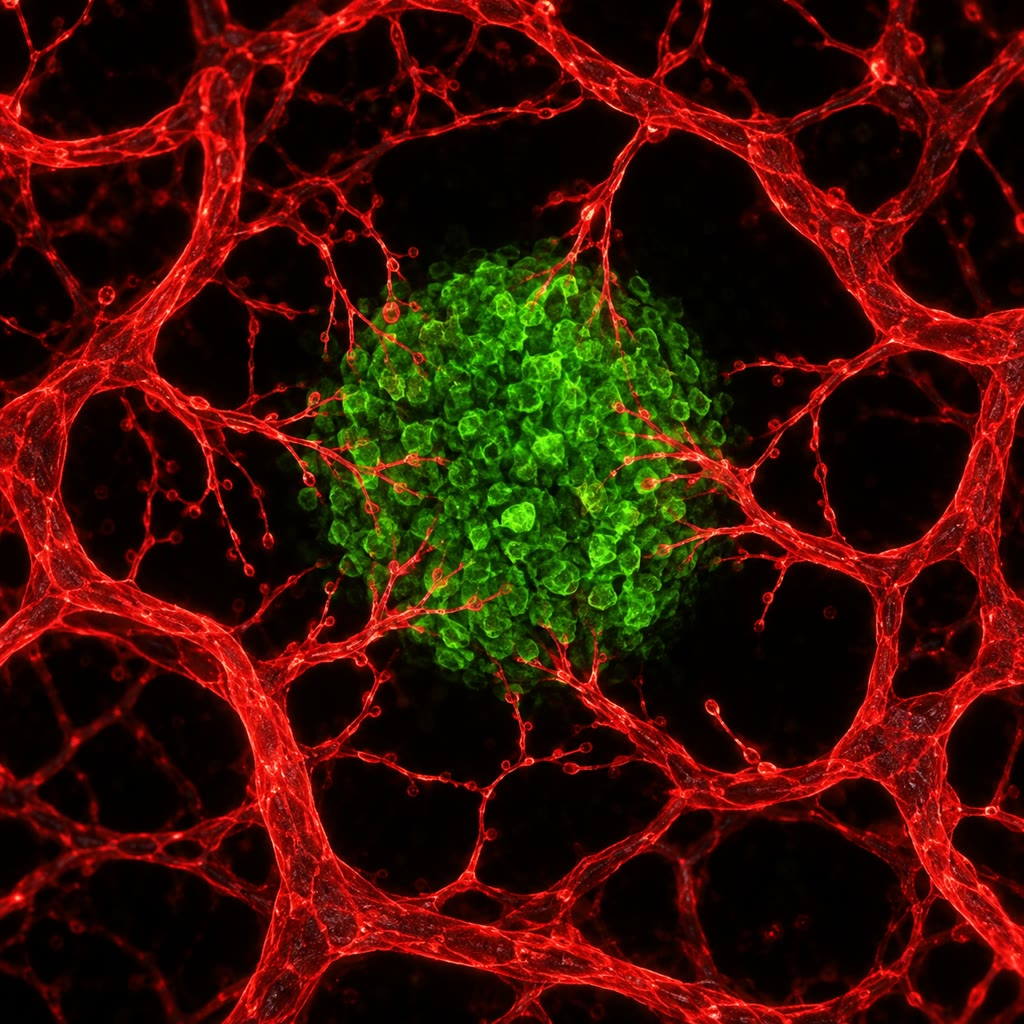
\includegraphics[width=0.36\linewidth]{images/book5/ai/b5-11-angiogenesis.jpg}\hspace{0.04\linewidth}
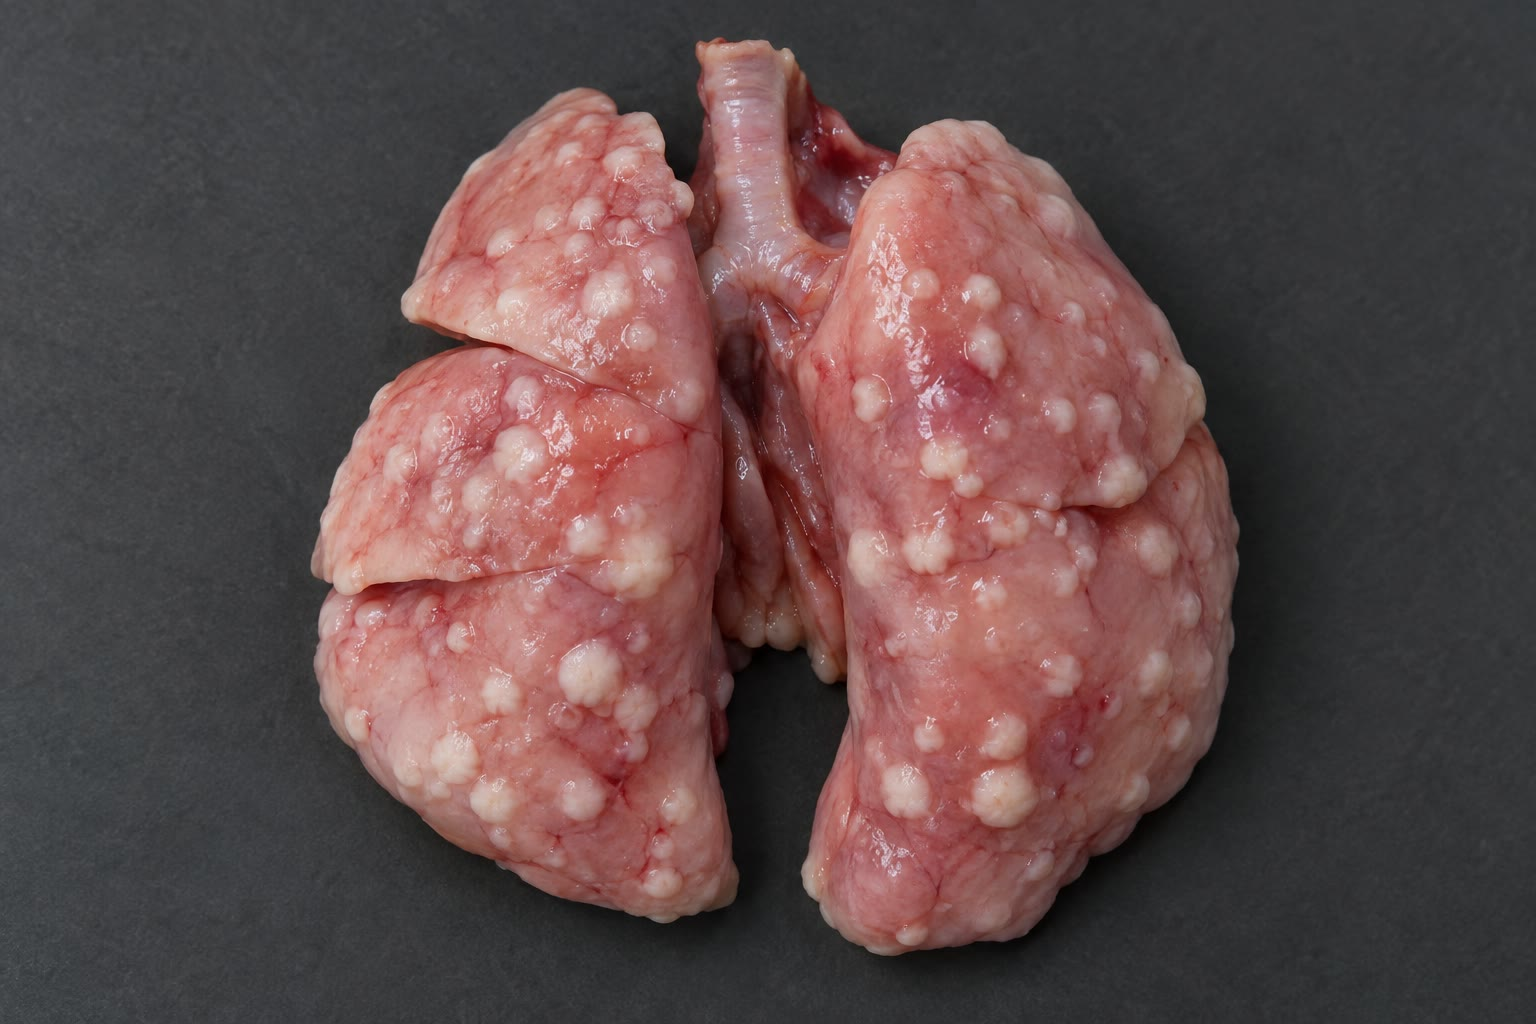
\includegraphics[width=0.54\linewidth]{images/book5/ai/b5-11-metastasis-lung.jpg}

{\small À esquerda: um esferoide tumoral (verde) recrutando vasos novos
(vermelho) de uma rede vizinha --- a angiogênese em cultura. À direita:
um pulmão de camundongo cravejado de \omterm{def:b3:cancer-biology:hallmarks}{metástases}, cada colônia fundada
por uma célula que sobreviveu à viagem pelo sangue.}
\end{omfigure}

\begin{definition}[Invasão e metástase]\label{def:b3:cancer-biology:metastasis}
\index{invasão}\index{transição epitélio--mesênquima}\index{semente e solo}
Para metastatizar, uma célula de carcinoma precisa deixar o epitélio
--- perder suas junções celulares e sua polaridade e adquirir
motilidade, uma \emph{transição epitélio--mesênquima} impulsionada por
fatores de transcrição normalmente usados no desenvolvimento
embrionário ---, degradar a membrana basal e a matriz com proteases
secretadas, atravessar a parede de um vaso sanguíneo ou linfático,
sobreviver na circulação (menos de uma em dez mil consegue, mortas pelo
cisalhamento, pela ausência de adesão e pelas células matadoras
naturais), alojar-se num leito capilar de outro órgão, sair dele e
crescer ali. Onde ela cresce não é aleatório: o \omterm{def:b3:cancer-biology:hallmarks}{câncer} de mama vai para
o osso, o pulmão, o fígado e o cérebro, o de cólon para o fígado, o de
próstata para o osso --- a \emph{semente e o solo} de Paget, de 1889,
explicados em parte pelo fluxo sanguíneo e em parte pelo ajuste entre a
célula e os sinais do tecido. Uma célula disseminada pode ficar
dormente por anos antes de crescer, e é por isso que os \omterm{def:b3:cancer-biology:hallmarks}{cânceres}
voltam uma década depois de uma cura aparente. A \omterm{def:b3:cancer-biology:hallmarks}{metástase} causa nove
em cada dez mortes por \omterm{def:b3:cancer-biology:hallmarks}{tumores} sólidos, e é a etapa menos compreendida.
\end{definition}

\begin{proposition}[Escapar do sistema imune]\label{prop:b3:cancer-biology:immune}
\index{evasão imune}\index{inibidor de ponto de checagem}\index{neoantígeno}
As mutações de um \omterm{def:b3:cancer-biology:hallmarks}{tumor} criam \emph{neoantígenos}, peptídeos que
nenhuma célula normal apresenta, e os linfócitos~T citotóxicos
reconhecem e matam células tumorais --- a razão pela qual pacientes
imunossuprimidos têm mais \omterm{def:b3:cancer-biology:hallmarks}{cânceres} e a razão pela qual os \omterm{def:b3:cancer-biology:hallmarks}{tumores} com
muitas mutações (melanoma, pulmão, cólon deficiente em \omterm{prop:b3:dna-repair:fidelity}{reparo de mau
pareamento}) respondem melhor à imunoterapia. Um \omterm{def:b3:cancer-biology:hallmarks}{tumor} clinicamente
evidente é um que escapou: perdendo as moléculas de MHC que apresentam
peptídeos, secretando fatores supressores, recrutando linfócitos~T
reguladores e, acima de tudo, expressando o PD-L1, que engata o
receptor inibitório PD-1 nos linfócitos~T e os desliga --- o mesmo
freio que normalmente encerra uma resposta imune
(\cref{ch:b3:adaptive-immunity}). Anticorpos que bloqueiam o PD-1 ou o
PD-L1, ou o freio anterior CTLA-4, soltam os linfócitos~T; numa fração
dos pacientes --- de um quinto a metade, conforme o \omterm{def:b3:cancer-biology:hallmarks}{tumor} --- eles
produzem remissões duradouras de \omterm{def:b3:cancer-biology:hallmarks}{cânceres} que eram intratáveis, e seus
efeitos colaterais são autoimunidade, a outra função do freio.
\end{proposition}

\section{Causas e tratamentos}

\begin{proposition}[Causas]\label{prop:b3:cancer-biology:causes}
\index{carcinógeno}\index{vírus oncogênico}
O \omterm{def:b3:cancer-biology:hallmarks}{câncer} é causado por tudo o que eleve a taxa dos eventos do teorema
ou o número de células sob risco. Os \emph{carcinógenos químicos}, a
maioria deles mutágenos depois da ativação pelo fígado: os setenta
carcinógenos da fumaça do tabaco, que causam um terço das mortes por
\omterm{def:b3:cancer-biology:hallmarks}{câncer} e elevam o risco de \omterm{def:b3:cancer-biology:hallmarks}{câncer} de pulmão de quinze a vinte e cinco
vezes; a aflatoxina de grãos mofados; o amianto, que não é mutágeno,
mas um irritante crônico. A \emph{radiação}: a luz ultravioleta para a
pele (os dímeros do \cref{ch:b3:dna-repair}), a radiação ionizante para
leucemia, tireoide e mama. As \emph{infecções}, um sexto dos \omterm{def:b3:cancer-biology:hallmarks}{cânceres}
no mundo: os papilomavírus, cujas proteínas E6 e E7 destroem a \omterm{def:b3:cancer-biology:genes}{p53} e
inativam a Rb e causam quase todos os \omterm{def:b3:cancer-biology:hallmarks}{cânceres} de colo do útero (uma
vacina hoje os previne); os vírus das hepatites B e C no \omterm{def:b3:cancer-biology:hallmarks}{câncer} de
fígado; o vírus Epstein--Barr em linfomas; o \emph{Helicobacter pylori}
no \omterm{def:b3:cancer-biology:hallmarks}{câncer} de estômago, por décadas de inflamação. As \emph{mutações
herdadas} num supressor de \omterm{def:b3:cancer-biology:hallmarks}{tumor}, o primeiro golpe já ao nascer, em
uns \qty{5}{\%} dos \omterm{def:b3:cancer-biology:hallmarks}{cânceres}. E o acaso: a maior parte das mutações de
um \omterm{def:b3:cancer-biology:hallmarks}{tumor} surgiu dos erros comuns da replicação, de modo que os tecidos
que mais se dividem --- cólon, pele, sangue --- têm mais \omterm{def:b3:cancer-biology:hallmarks}{cânceres}, e o
risco sobe com a idade faça-se o que fizer.
\end{proposition}

\begin{theorem}[Por que um fármaco falha e dois podem não falhar]\label{thm:b3:cancer-biology:goldie-coldman}
\index{modelo de Goldie--Coldman}\index{resistência a fármacos}\index{terapia combinada}
Seja um \omterm{def:b3:cancer-biology:hallmarks}{tumor} de $N$ células produzido por divisões sucessivas a partir
de uma célula, e seja $\mu$ a taxa com que surge, por divisão celular,
uma mutação que confere resistência a um dado fármaco. Então a
probabilidade de o \omterm{def:b3:cancer-biology:hallmarks}{tumor} \emph{não} conter célula resistente alguma
quando o tratamento começa é de cerca de
\[
P_{0} \approx e^{-\mu N},
\]
de modo que, para $\mu N \gg 1$, a resistência preexiste com quase
certeza. Para dois fármacos com mecanismos de resistência
independentes, uma célula resistente aos dois surge a uma taxa de cerca
de $\mu_{1}\mu_{2}$ por divisão, e $P_{0}
\approx e^{-\mu_{1}\mu_{2}N}$:
com $N = 10^{9}$ e $\mu = 10^{-7}$, um fármaco enfrenta $\mu N = 100$
clones resistentes em média, e dois fármacos, uma probabilidade de
$10^{-5}$ de existir sequer uma célula duplamente resistente.
\end{theorem}
\begin{proof}[Prova parcial]
Crescer de $1$ a $N$ células leva cerca de $N$ divisões ao todo (uma
árvore com $N$ folhas tem $N - 1$ nós internos). Se uma célula
resistente é produzida a cada divisão com probabilidade $\mu$ e, numa
primeira aproximação, seus descendentes não morrem nem superam os
demais, o número de eventos de resistência é Poisson de média $\mu N$,
e a probabilidade de nenhum é $e^{-\mu N}$. Mecanismos independentes
multiplicam as probabilidades por divisão. A aproximação despreza o
fato de que mutantes precoces deixam clones resistentes maiores --- a
distribuição completa é a de Luria e Delbrück, tratada no volume do
2.º ano ---, mas a probabilidade de \emph{nenhum} mutante, que é o que
decide se o \omterm{def:b3:cancer-biology:hallmarks}{tumor} pode ser curado, é exatamente o termo de Poisson.
\end{proof}

\begin{example}[As terapias e sua lógica]\label{ex:b3:cancer-biology:therapy}
A cirurgia e a radioterapia removem ou matam um \omterm{def:b3:cancer-biology:hallmarks}{tumor} localizado; a
radiação mata por \omterm{def:b3:dna-repair:lesions}{quebras de fita dupla}, e seu fracionamento em doses
diárias deixa o tecido normal reparar entre elas
(\cref{ch:b3:dna-repair}). A quimioterapia citotóxica --- agentes
alquilantes, antimetabólitos, venenos de \omterm{def:b3:cytoskeleton-motility:filaments}{microtúbulos}, inibidores de
topoisomerase --- mata células em divisão de qualquer tipo, as
tumorais um pouco mais, e segue uma lei de \emph{morte logarítmica}:
cada ciclo mata uma fração constante, digamos \qty{99}{\%}, de modo que
seis ciclos reduzem $10^{12}$ células a uma, e os mesmos seis ciclos
são necessários seja o \omterm{def:b3:cancer-biology:hallmarks}{tumor} grande ou pequeno; o cabelo, o intestino e
a medula do paciente, que também se dividem, fixam a dose. A terapia
alvo ataca uma lesão de que o \omterm{def:b3:cancer-biology:hallmarks}{tumor} depende: o imatinibe bloqueia a
cinase BCR--ABL e converteu a leucemia mieloide crônica de uma doença
fatal numa doença crônica; o trastuzumabe se liga ao HER2; os
inibidores de PARP, os inibidores de Cdk4/6 e o venetoclax dos
capítulos anteriores exploram, cada um, um defeito. A imunoterapia
solta os linfócitos~T. E o teorema diz como devem ser usados: em
combinação, cedo, quando $N$ é menor --- que é o que faz a quimioterapia
adjuvante depois da cirurgia --- e com fármacos cujos mecanismos de
resistência não se sobreponham. O \omterm{def:b3:cancer-biology:hallmarks}{tumor} é uma população em evolução, e
o tratamento é seleção.
\end{example}

\begin{omfigure}
\begin{tikzpicture}
\begin{axis}[
  width=0.7\linewidth, height=5.6cm,
  axis x line=bottom, axis y line=left,
  xmin=0, xmax=8, ymin=1, ymax=1e13, ymode=log,
  xlabel={ciclos de quimioterapia}, ylabel={células tumorais},
  xlabel style={font=\small, at={(axis description cs:0.5,-0.12)}, anchor=north},
  ylabel style={font=\small},
  tick label style={font=\small}, xtick={0,2,4,6,8},
  clip=false,
]
\addplot[very thick, omDef, mark=*, mark size=1.2pt] coordinates {(0,1e12) (1,1e10) (2,1e8) (3,1e6) (4,1e4) (5,1e2) (6,1)};
\addplot[very thick, omThm, mark=*, mark size=1.2pt] coordinates {(0,1e12) (1,1.01e10) (2,1.02e8) (3,1.04e6) (4,1.1e4) (5,200) (6,300) (7,600) (8,1200)};
\addplot[dashed, gray, domain=0:8, samples=2] {1e9};
\node[font=\scriptsize, gray, anchor=south west] at (axis cs:0.2,1.3e9) {detectável, $10^{9}$};
\node[font=\scriptsize, omDef, anchor=south west] at (axis cs:0.3,1e4) {\qty{99}{\%} de morte por ciclo};
\node[font=\scriptsize, omThm, anchor=south west] at (axis cs:5.2,3e3) {uma célula resistente no início: recidiva};
\end{axis}
\end{tikzpicture}

{\small A lei da morte logarítmica. Cada ciclo mata a mesma fração de
células, de modo que o \omterm{def:b3:cancer-biology:hallmarks}{tumor} encolhe um número fixo de décadas por
ciclo e fica indetectável muito antes de ter acabado (azul); uma única
célula resistente preexistente sobrevive a cada ciclo e volta a crescer
(vermelho).}
\end{omfigure}

\begin{remark}[O que mudou]\label{rem:b3:cancer-biology:changed}
Metade de todos os pacientes diagnosticados com \omterm{def:b3:cancer-biology:hallmarks}{câncer} num país rico
sobrevive hoje dez anos, contra um quarto em 1970. O ganho veio da
prevenção (tabaco, vacinas contra hepatite e papilomavírus, rastreio de
pólipos e de lesões do colo do útero), da detecção mais precoce e de
tratamentos que decorrem da biologia deste capítulo --- a quimioterapia
combinada que cura a maioria das leucemias da infância e dos \omterm{def:b3:cancer-biology:hallmarks}{cânceres}
de testículo, os fármacos-alvo e as imunoterapias. O que não mudou foi
a doença metastática, que a biologia explica, mas ainda não cura; os
próximos ganhos virão de tratar o \omterm{def:b3:cancer-biology:hallmarks}{tumor} pelo que ele é, uma população
em evolução sob a seleção que o tratamento impõe.
\end{remark}

\section{Exercícios}

\begin{exercise}[$\star$]\label{exo:b3:cancer-biology:1}
Distinga um \omterm{def:b3:cancer-biology:genes}{oncogene} de um \omterm{def:b3:cancer-biology:genes}{gene supressor de tumor} quanto ao mecanismo
e ao número de alelos que precisam mudar, com dois exemplos de cada.
\end{exercise}

\begin{exercise}[$\star$]\label{exo:b3:cancer-biology:2}
Liste as \omterm{def:b3:cancer-biology:hallmarks}{marcas do câncer} e, para cada uma, nomeie um gene deste ou de
um capítulo anterior cuja alteração a fornece.
\end{exercise}

\begin{exercise}[$\star$]\label{exo:b3:cancer-biology:3}
O que Knudson observou sobre o retinoblastoma hereditário e o
esporádico, e o que ele inferiu?
\end{exercise}

\begin{exercise}[$\star$]\label{exo:b3:cancer-biology:4}
Explique o \omterm{met:b3:cancer-biology:ames}{teste de Ames} e por que um extrato de fígado é acrescentado.
\end{exercise}

\begin{exercise}[$\star\star$]\label{exo:b3:cancer-biology:5}
A incidência de um \omterm{def:b3:cancer-biology:hallmarks}{câncer} é $2\times 10^{-5}$ por ano aos $40$ anos e
$2\times 10^{-3}$ aos $80$. Estime o expoente da lei de potência da
idade e o número de eventos limitantes da taxa que ele sugere.
\end{exercise}

\begin{exercise}[$\star\star$]\label{exo:b3:cancer-biology:6}
Usando a \cref{prop:b3:cancer-biology:oxygen} com
$D =
\qty{2e-9}{m^2/s}$ e $c_{0} = \qty{0.05}{mol/m^3}$, calcule $L$
para um tecido que consome \qty{0.01}{mol/m^3/s} e para um \omterm{def:b3:cancer-biology:hallmarks}{tumor} que
consome três vezes mais. Por que um \omterm{def:b3:cancer-biology:hallmarks}{tumor} de crescimento rápido se
torna necrótico mais cedo?
\end{exercise}

\begin{exercise}[$\star\star$]\label{exo:b3:cancer-biology:7}
Um \omterm{def:b3:cancer-biology:hallmarks}{tumor} de $10^{11}$ células é tratado com um fármaco que mata
\qty{99.9}{\%} por ciclo. Quantos ciclos para reduzi-lo a menos de uma
célula? Por que o \omterm{def:b3:cancer-biology:hallmarks}{tumor} fica indetectável depois de dois ciclos, embora
restem $10^{5}$ células, e o que isso implica para a interrupção do
tratamento?
\end{exercise}

\begin{exercise}[$\star\star$]\label{exo:b3:cancer-biology:8}
Explique por que uma mutação no EGFR e uma mutação no KRAS raramente
são encontradas no mesmo \omterm{def:b3:cancer-biology:hallmarks}{tumor} de pulmão, e por que um \omterm{def:b3:cancer-biology:hallmarks}{tumor} tratado
com um inibidor de EGFR muitas vezes recidiva com uma mutação em KRAS.
\end{exercise}

\begin{exercise}[$\star\star$]\label{exo:b3:cancer-biology:9}
As proteínas E6 e E7 do papilomavírus inativam a \omterm{def:b3:cancer-biology:genes}{p53} e a Rb. Explique
como isso impulsiona o \omterm{def:b3:cancer-biology:hallmarks}{câncer} de colo do útero, por que isso leva
décadas, e por que uma vacina dada antes da atividade sexual o previne.
\end{exercise}

\begin{exercise}[$\star\star\star$]\label{exo:b3:cancer-biology:10}
Estenda o argumento de Armitage--Doll para permitir que cada golpe
expanda seu clone por um fator $g$ antes do seguinte: mostre que a
incidência tem a mesma potência de $t$, mas um prefator multiplicado
por $g^{k-1}$, e discuta por que o $k$ ajustado a partir de uma curva
de idade é um limite superior do número de condutoras.
\end{exercise}

\begin{exercise}[$\star\star\star$]\label{exo:b3:cancer-biology:11}
Com o \cref{thm:b3:cancer-biology:goldie-coldman}, compare (a) tratar um
\omterm{def:b3:cancer-biology:hallmarks}{tumor} de $10^{9}$ células com o fármaco A por seis ciclos e depois com
o fármaco B por seis, e (b) dar A e B juntos desde o início, quando
$\mu_{A} =
\mu_{B} = 10^{-7}$. Calcule $P_{0}$ para cada estratégia e
explique por que a combinação precoce é a regra.
\end{exercise}

\begin{exercise}[$\star\star\star$]\label{exo:b3:cancer-biology:12}
O paradoxo de Peto: um elefante tem cem vezes mais células que um
humano e vive o mesmo tanto, e ainda assim não tem mais \omterm{def:b3:cancer-biology:hallmarks}{câncer}. Usando
o teorema deste capítulo, diga qual é a expectativa ingênua e proponha
dois mecanismos pelos quais os animais grandes poderiam ter resolvido o
problema (o elefante tem vinte cópias do \emph{TP53}).
\end{exercise}

\section{Problema: a aritmética de um tumor}

\begin{problem}[{Problema de fim de semana --- um tumor crescido a
partir de uma célula e cronometrado até a detecção, sua curva de idade
lida em busca do número de golpes, seu suprimento de oxigênio e seu
núcleo necrótico calculados, e seu tratamento planejado contra a
certeza da resistência, terminando nos anos até a detecção, na
profundidade de tumor vivo em torno de um vaso e na probabilidade de
uma combinação curar}]
\label{pb:b3:cancer-biology:1}
Dados: uma célula tumoral tem volume \qty{1000}{\micro m^3}; tempo de
duplicação \qty{100}{d}; detecção a \qty{1}{cm^3}; carga letal
\qty{1}{kg}. Curva de idade: incidência $1\times 10^{-5}$ por ano aos
$30$ e $3\times
10^{-3}$ aos $80$. Oxigênio: $D = \qty{2e-9}{m^2/s}$,
$c_{0} =
\qty{0.05}{mol/m^3}$, $q = \qty{0.03}{mol/m^3/s}$ no \omterm{def:b3:cancer-biology:hallmarks}{tumor}; os
capilares de um \omterm{def:b3:cancer-biology:hallmarks}{tumor} vascularizado estão a \qty{150}{\micro m} um do
outro. Terapia: cada ciclo mata \qty{99}{\%}; taxa de mutação de
resistência $10^{-7}$ por divisão por fármaco; um ciclo a cada três
semanas; o \omterm{def:b3:cancer-biology:hallmarks}{tumor} volta a crescer entre os ciclos com o mesmo tempo de
duplicação.

\medskip
\noindent\textbf{Parte I --- Crescimento.}
\begin{enumerate}
  \item Quantas células há em \qty{1}{cm^3}? Quantas duplicações a
        partir de uma célula?
  \item Quantos anos da célula fundadora até a detecção?
  \item Quantas duplicações, e quantos anos, da detecção até a carga
        letal? Compare os dois intervalos.
  \item Muitos \omterm{def:b3:cancer-biology:hallmarks}{tumores} são detectados a \qty{1}{cm^3}, mas cresciam
        havia apenas cinco anos. O que precisa ter sido verdade a
        respeito do tempo de duplicação no início, ou da lei de
        crescimento?
  \item Apenas uma fração $f$ das células de um \omterm{def:b3:cancer-biology:hallmarks}{tumor} está em divisão a
        cada momento (a fração de crescimento), e uma fração morre. Se
        as células ciclam em \qty{2}{d}, mas o \omterm{def:b3:cancer-biology:hallmarks}{tumor} duplica em
        $100$, o que isso diz sobre o balanço entre nascimento e morte?
  \item Por que a mesma quimioterapia de morte logarítmica poupa mais
        um \omterm{def:b3:cancer-biology:hallmarks}{tumor} de crescimento lento que um rápido, e, ainda assim, o
        rápido volta a crescer mais depressa entre os ciclos?
\end{enumerate}

\medskip
\noindent\textbf{Parte II --- Golpes.}
\begin{enumerate}[resume]
  \item A partir das duas incidências, calcule o expoente $k - 1$ da
        curva de idade e o número implícito de eventos $k$.
  \item Se cada evento ocorre a $u = 10^{-6}$ por célula por ano em
        $N = 10^{8}$ células suscetíveis, o que o teorema prevê para o
        risco cumulativo até os $70$ anos com o seu $k$? É plausível? O
        que está faltando?
  \item Repita com uma expansão clonal por um fator $g = 100$ depois de
        cada um dos primeiros $k - 1$ golpes, usando o
        \cref{exo:b3:cancer-biology:10}.
  \item Uma portadora herda um golpe. Por qual fator sua incidência aos
        $40$ anos é elevada, se as outras taxas não mudam? (Compare
        $(ut)^{k-1}$ com $(ut)^{k}$ em $t = 40$.)
  \item Fumar multiplica o $u$ de um dos eventos por $10$. Por qual
        fator a incidência sobe se esse evento é um dos $k$; e se forem
        dois deles?
  \item Explique por que parar de fumar aos cinquenta baixa o risco de
        \omterm{def:b3:cancer-biology:hallmarks}{câncer} de pulmão abaixo do de um fumante que continua, mas
        nunca ao de quem nunca fumou.
\end{enumerate}

\medskip
\noindent\textbf{Parte III --- Suprimento.}
\begin{enumerate}[resume]
  \item Calcule a profundidade de penetração do oxigênio $L$ no \omterm{def:b3:cancer-biology:hallmarks}{tumor}.
  \item Um esferoide sem vasos: qual é o diâmetro máximo em que cada
        célula está oxigenada? Qual é a espessura da borda viva de um
        esferoide de \qty{2}{mm}, e que fração de seu volume está viva?
  \item Num \omterm{def:b3:cancer-biology:hallmarks}{tumor} vascularizado com capilares a \qty{150}{\micro m} um
        do outro, cada célula está oxigenada? Quais células estão
        hipóxicas, e por que isso importa para a radioterapia (o
        oxigênio fixa o dano da radiação) e para a seleção de células
        com \omterm{def:b3:cancer-biology:genes}{p53} mutante?
  \item Um fármaco reduz à metade a densidade de capilares do \omterm{def:b3:cancer-biology:hallmarks}{tumor}.
        Recalcule o espaçamento e diga o que acontece com as células a
        meio caminho entre os vasos.
  \item As células hipóxicas passam à glicólise, fazendo \qty{2}{ATP}
        por glicose em vez de $30$. Por qual fator elas precisam elevar
        a captação de glicose para manter seu suprimento de ATP, e como
        isso é explorado na imagem de \omterm{def:b3:cancer-biology:hallmarks}{tumores}?
  \item Explique por que a terapia antiangiogênica sozinha raramente
        cura, mas pode ajudar a quimioterapia a alcançar o \omterm{def:b3:cancer-biology:hallmarks}{tumor}.
\end{enumerate}

\medskip
\noindent\textbf{Parte IV --- Tratamento.}
\begin{enumerate}[resume]
  \item Um \omterm{def:b3:cancer-biology:hallmarks}{tumor} de \qty{1}{cm^3} é tratado com um fármaco. Quantos
        ciclos o reduzem a menos de uma célula, ignorando o
        recrescimento e a resistência?
  \item Entre os ciclos (três semanas) os sobreviventes voltam a
        crescer. Por qual fator? Recalcule a morte líquida por ciclo e o
        número de ciclos necessários.
  \item Calcule o número esperado de células resistentes ao fármaco no
        início do tratamento e a probabilidade de não haver nenhuma.
  \item Dois fármacos com mecanismos independentes são dados juntos.
        Probabilidade de não existir célula duplamente resistente no
        início? E num \omterm{def:b3:cancer-biology:hallmarks}{tumor} de $10^{12}$ células?
  \item A terapia adjuvante é dada depois da cirurgia, quando talvez
        $10^{6}$ células permaneçam sem ser detectadas. Recalcule as
        probabilidades para um e para dois fármacos e enuncie a lição.
  \item Uma imunoterapia induz linfócitos~T que matam qualquer célula
        que apresente um neoantígeno. Por que a resistência a ela é um
        problema diferente da resistência a um inibidor de cinase, e em
        quais \omterm{def:b3:cancer-biology:hallmarks}{tumores} o teorema sugere que ela deva funcionar melhor?
  \item Resuma: os anos da célula fundadora até a detecção (questão~2),
        a profundidade de \omterm{def:b3:cancer-biology:hallmarks}{tumor} vivo em torno de um vaso (questão~13) e
        a probabilidade de a combinação de dois fármacos não enfrentar
        célula resistente alguma num \omterm{def:b3:cancer-biology:hallmarks}{tumor} de \qty{1}{cm^3}
        (questão~22).
\end{enumerate}
\end{problem}
